\documentclass[11pt,a4paper]{article}
\usepackage[margin=2.5cm]{geometry}
\usepackage[utf8]{inputenc}
\usepackage[T1]{fontenc}
\usepackage{hyperref}
\renewcommand{\familydefault}{\sfdefault}
\usepackage{helvet}
\pagestyle{empty}
\usepackage[kerning=true]{microtype}
\usepackage{parskip}
\usepackage{sansmath}
\usepackage[font={small, bf}]{caption}
\usepackage[font={small}]{subcaption}
\usepackage{graphicx}
\usepackage{multicol}
\setlength{\abovecaptionskip}{0pt}
\setlength{\floatsep}{10pt}
\setlength{\textfloatsep}{0pt}
\setlength{\intextsep}{0pt}
\setlength{\belowcaptionskip}{0pt}
\setlength{\parindent}{5ex}
\setlength{\parskip}{0pt}
% Feel free to use additional packages for glosses, figures, whatnot.

% The next bit is for reserving sufficient space for authors,
% affiliations, and e-mail address.  No need to change for initial
% anonymous version.  For the final version, replace the
% \toggletrue{anonymous} with \togglefalse{anonymous} to de-anonymize.
\usepackage{etoolbox}
\newtoggle{anonymous}
\togglefalse{anonymous}

\renewcommand{\title}[1]{\textbf{#1}\\}
\newcommand{\authors}[1]{\iftoggle{anonymous}{\phantom{#1}}{#1}\\}
\newcommand{\email}[1]{\iftoggle{anonymous}{\phantom{#1}}{#1}}

\begin{document}

% First page:

% Insert title, authors, affiliations, and e-mail address in the next three lines:

\title{TODO}
\authors{Veronica Boyce, Robert Hawkins, Noah Goodman, Michael C. Frank} 
\email{vboyce@stanford.edu}
\newline
%

% Intro
%TODO citations
Shared referring expressions are a necessity for efficient communication; when there are not widely shared conventional names for objects, people must create spontaneous ad-hoc expressions. The formation and adoption of these new reference expressions is well-studied in dyadic contexts where one speaker refers to a set of images repeatedly to one listener. Over repetition, a few key phenomena emerge: listener's have high and increasing target accuracy while speaker's descriptions shorten as nicknames develop; crucially, these reduced referring expressions are partner-specific; dyads converge to nicknames, but dyads diverge from other dyads. This leaves a question of how well it generalizes to larger groups and what properties of the communication channel are necessary for the pattern to emerge.  TODO citations

\textbf{Methods:} We explore this with a 2x2 design crossing group size (2 or 6 players) with communication channel width. In \textbf{thick} games (maximizing effective communication channel), the same player will be the speaker the entire time, all listeners will be able to use the chat to ask questions, and all players will see who selected what and whether it was right. In the \textbf{thin} condition, the speaker role will rotate by block, the speaker will use the chat while listeners will be limited to sending 4 emojis as backchannel options, and each listener will only see feedback on their own selection. 

We recruited participants from Prolific to do this experiment as a real-time interactive game written in Empirica (Almaatouq et al. 2021). As shown in Figure 1,  participants see 12 tangram figures, one of which is indicated to the speaker, who describes the target to the listeners, who click on their selection.  At the end of the trial feedback is given.  After all 12 tangrams have been described, the process repeats, for a total of 6 blocks (72 referential trials). We had roughly 40 games in each of the 4 conditions, for a total of 623 participants and 160K words. 

% Results

\textbf{Results:} In line with prior work, we find increasing listener accuracy and decreasing utterance lengths over the course of the game (Figs 2A and B). There are also condition differences. While speakers tend to say less later in all games, speakers use fewer words in 2 player games compared to 6 player games throughout blocks.  All conditions show high and increasing accuracy, but both group size and channel width affect accuracy: 2 person groups and thick channels have high accuracy. 



To analyze linguistic content, we embed the speaker's utterances with S-BERT (Reimers \& Gurevych 2020) to map the speaker's language on each trial to a vector in high-dimensional semantic space. We then use cosine similarity between pairs of vectors as a proxy for similarity between pairs of utterances. To look for group differentiation, we take cosine similarities between descriptions of the same tangram in the same block in different games. If each group develops partner-specific nicknames, we expect decreasing similarity over blocks. We find this pattern 2 player games and 6 player thick games (Fig 2C). The 6 player thin condition shows a much flatter pattern, suggesting less specialization. 

To measure within group convergence to a shared convention, we treat final block utterances as the ``convention'' and measure the cosine similarity between earlier utterances in the same game for the same tangram to this final ``convention''. If there is convergence to a convention, we expect similarity to the convention to increase over blocks. We find increasing similarity across conditions, and games in the thick condition 2 player games increase faster and more strongly, indicating faster convergence to a nickname (Fig 2D). 

\textbf{Conclusion:} We show that participants can still achieve high levels of accuracy even with multiple partners and limited communication channel; however, this condition does not show convergence to a shared, partner-specific conventional nickname. These condition manipulations being to suggest what aspects of communication are necessary for the dyadic repeated reference phenomena.

\newpage

\begin{figure}
	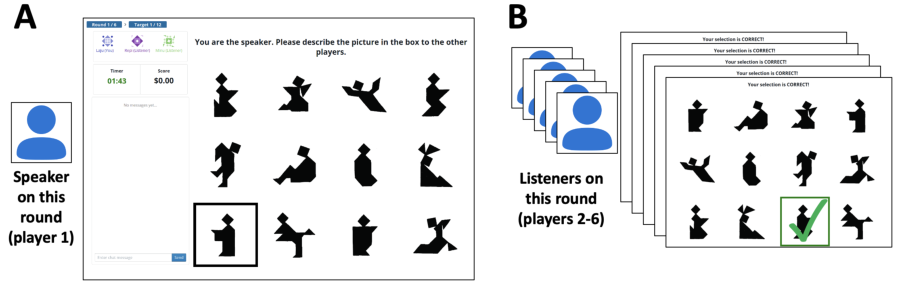
\includegraphics[width=\textwidth]{../images/interface-1.pdf}
	\caption{Schematic of player interface}
\end{figure}

\begin{figure}
	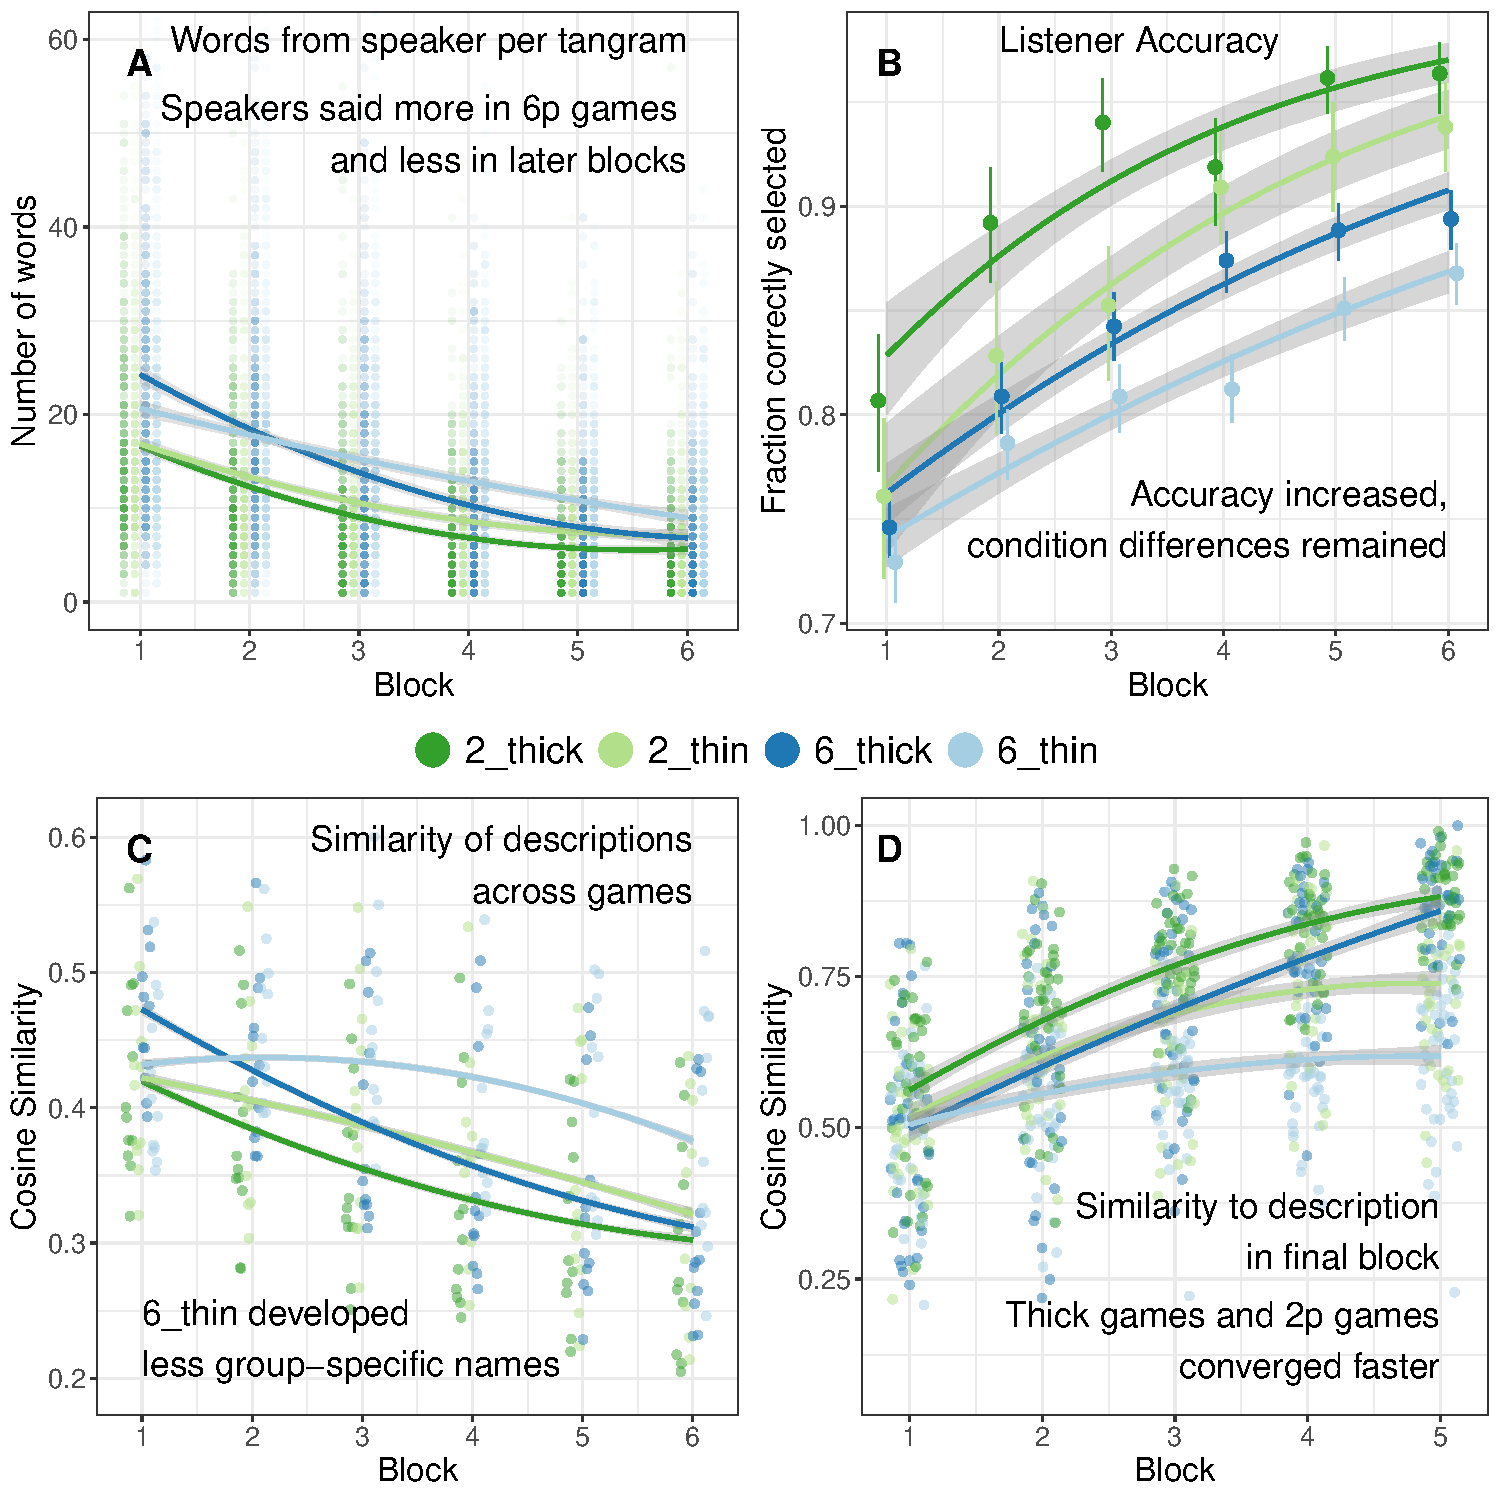
\includegraphics[width=\textwidth]{../images/CAMP1.pdf}
	\caption{Results by condition}
\end{figure}

\begin{figure} \textbf{References:} Reimers \& Gurevych EMNLP 2020. $\bullet$ Almaatouq et al. Behav. Res. Methods 2021. \end{figure}

\end{document}